\documentclass{article}
\usepackage[utf8]{inputenc}
\usepackage[spanish]{babel}
\usepackage{graphicx}
\usepackage{geometry}
\usepackage{amsmath}
\usepackage{float}
\usepackage{setspace}
\usepackage{lmodern}
\usepackage{booktabs}
\usepackage{array}

\geometry{a4paper, margin=1in}
\setlength{\parskip}{0.5em}
\onehalfspacing
\title{Análisis de Regresión Logística}
\author{Cristian Ernesto Antonio Santiago}
\date{}

\begin{document}

\maketitle

\section{Introducción}

La regresión logística es un algoritmo fundamental en el aprendizaje automático, diseñado para problemas de clasificación donde la variable objetivo es categórica. A diferencia de la regresión lineal que predice valores continuos, este método estima probabilidades pertenecientes a categorías específicas mediante una función sigmoide, la cual transforma las salidas a un rango entre 0 y 1. Su nombre, aunque sugiere similitud con la regresión lineal, responde a su uso de la función logística para modelar relaciones no lineales entre variables.

En el contexto de clasificación de sistemas operativos, la regresión logística resulta ideal por su capacidad para manejar múltiples variables predictoras (como tiempo de sesión, páginas visitadas o tipo de dispositivo) y asignar probabilidades a cada categoría (Windows, Macintosh o Linux). El modelo calcula la probabilidad de que un usuario pertenezca a cada clase, seleccionando finalmente la de mayor probabilidad.

Su importancia radica en tres aspectos clave: interpretabilidad (los coeficientes indican cómo cada variable afecta la clasificación), eficiencia computacional (ideal para conjuntos de datos medianos) y versatilidad (aplicable desde diagnóstico médico hasta análisis de marketing digital). Para el caso de uso planteado, permitirá identificar patrones de navegación asociados a cada sistema operativo, ofreciendo insights valiosos para personalización de contenido o detección de anomalías.

El modelo multivariante extiende esta lógica a múltiples categorías mediante técnicas como \textit{one-vs-rest}, donde se entrenan clasificadores binarios independientes para cada clase. Esto lo convierte en una herramienta poderosa para problemas como el planteado, donde los usuarios pueden clasificarse en tres categorías mutuamente excluyentes basadas en su comportamiento digital.

\newpage

\section{Metodología}

\subsection*{Configuración inicial y carga de datos}

\begin{figure}[H]
\centering
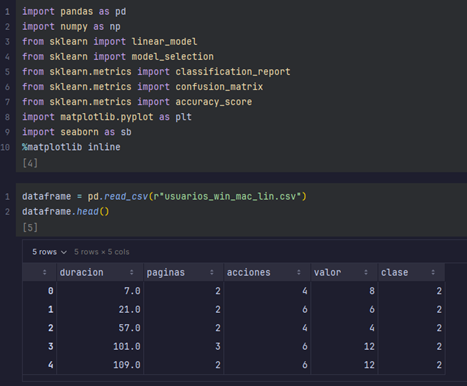
\includegraphics[width=1.0\textwidth]{Actividad-11/Imagen1.png}
\end{figure}

Primero se importaron las librerías esenciales para el análisis. \textit{Pandas} y \textit{NumPy} se utilizaron para la manipulación de datos, mientras que las funciones de \textit{Scikit-learn} permitieron implementar el modelo de clasificación. Para la evaluación, se importaron métricas clave como  \textit{classification\_report}, \textit{confusion\_matrix} y \textit{accuracy\_score}. Las librerías \textit{Matplotlib} y \textit{Seaborn} se incluyeron para generar visualizaciones, con la configuración \texttt{\%matplotlib inline }para mostrar los gráficos directamente en el entorno de trabajo.

Luego se cargó el dataset mediante \textit{pd.read\_csv()}, leyendo el archivo "usuarios\_win\_mac\_lin.csv" que contiene registros de comportamiento de usuarios. La función \textit{head()} mostró los primeros cinco registros, revelando la estructura básica del dataset. Se observaron columnas como:

\begin{itemize}
    \item \textbf{duración:} Tiempo de sesión en minutos
    \item \textbf{paginas:} Número de páginas visitadas
    \item \textbf{acciones:} Interacciones realizadas
    \item \textbf{valor:} Puntuación de comportamiento
    \item \textbf{clase:} Variable objetivo (sistema operativo)
\end{itemize}

\section*{Análisis estadístico exploratorio}

\begin{figure}[H]
\centering
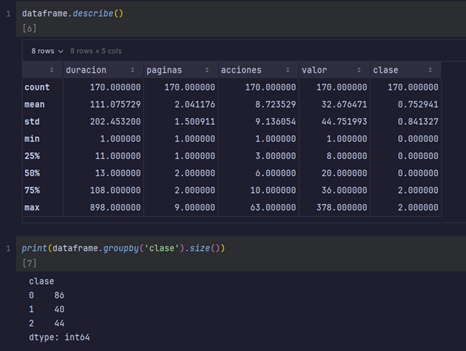
\includegraphics[width=0.9\textwidth]{Actividad-11/Imagen2.png}
\end{figure}

Primero se examinaron las estadísticas descriptivas del dataset mediante \textit{dataframe.describe()}, lo que reveló información clave sobre la distribución de las variables. Los resultados mostraron que el tiempo de sesión (\textit{duración}) presenta una amplia variabilidad (de 1 a 898 minutos), con una media de 111 minutos pero una mediana de solo 13 minutos, indicando una distribución altamente asimétrica donde pocas sesiones prolongadas elevan el promedio. Las páginas visitadas (\textit{paginas}) se concentran mayormente entre 1 y 2, mientras que las interacciones (\textit{acciones}) y el valor de comportamiento muestran rangos más amplios.

Posteriormente, al analizar la distribución de clases con groupby('clase').size(), se identificó un desbalance moderado en los datos: la clase 0 (Windows) domina con 86 instancias, frente a 40 de clase 1 (Mac) y 44 de clase 2 (Linux). Esta distribución desigual podría afectar el rendimiento del clasificador para las categorías minoritarias, aspecto que deberá considerarse durante el entrenamiento del modelo.

\section*{Visualización de distribuciones de características}

\begin{figure}[H]
\centering
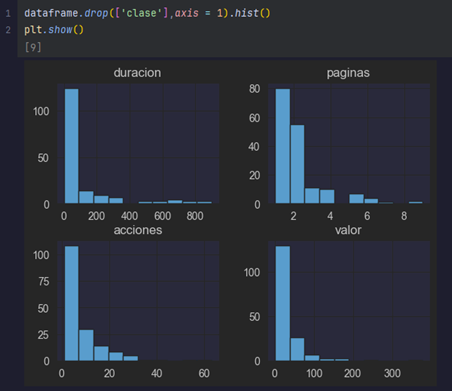
\includegraphics[width=0.9\textwidth]{Actividad-11/Imagen3.png}
\end{figure}

Para complementar el análisis numérico previo, se generaron histogramas de las variables predictoras mediante dataframe.drop(['clase'],axis=1).hist(). Esta operación eliminó primero la columna objetivo ('clase') para enfocarse únicamente en las características de entrada, generando una matriz de gráficos donde cada subplot muestra la distribución de una variable.

Los histogramas revelaron patrones importantes: la duración de sesión ('duracion') presenta una distribución extremadamente sesgada, con la mayoría de valores concentrados cerca del cero pero con algunos casos que se extienden hasta 800 minutos. El número de páginas visitadas ('paginas') muestra un comportamiento discreto, con picos en valores enteros (especialmente 1 y 2 páginas). Por otro lado, las acciones ('acciones') y el valor ('valor') exhiben distribuciones más dispersas, aunque con una clara asimetría positiva donde la mayoría de registros se agrupan en los valores bajos.

Esta visualización confirmó la necesidad detectada en el análisis estadístico previo: varias variables requerirán transformación (como normalización logarítmica para 'duracion') para mejorar el rendimiento del modelo de clasificación. La heterogeneidad en las escalas de las características también sugiere que será crucial aplicar estandarización antes del entrenamiento.

\newpage

\section*{Análisis multivariable de relaciones entre características}

\begin{figure}[H]
\centering
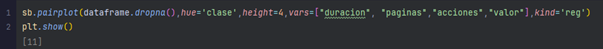
\includegraphics[width=0.9\textwidth]{Actividad-11/Imagen4.png}
\end{figure}

El código implementó una visualización avanzada mediante sb.pairplot(), creando una matriz de gráficos que combina histogramas y regresiones lineales para examinar las relaciones entre las variables predictoras, diferenciadas por color según la clase de sistema operativo. Esta técnica permite identificar patrones complejos que los análisis univariados previos no podían revelar.

\begin{figure}[H]
\centering
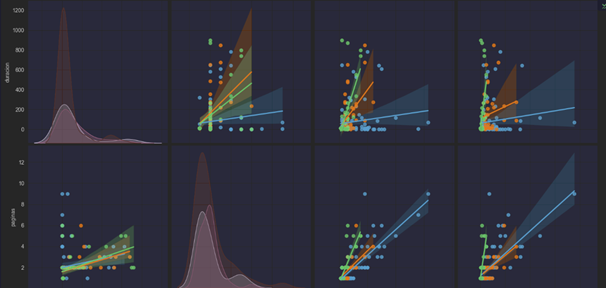
\includegraphics[width=0.9\textwidth]{Actividad-11/Imagen5.png}
\end{figure}

\begin{figure}[H]
\centering
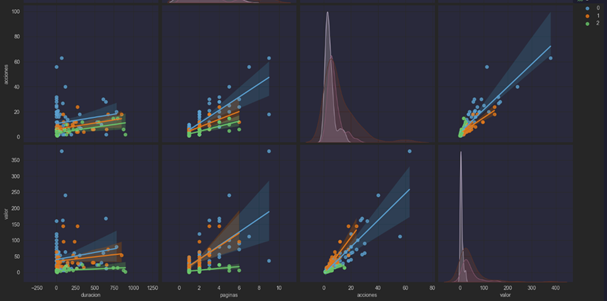
\includegraphics[width=0.9\textwidth]{Actividad-11/Imagen6.png}
\end{figure}

En los gráficos generados, se observaron varias relaciones clave:

\begin{itemize}
    \item \textbf{Duración vs páginas visitadas:} Mostró una ligera correlación positiva, particularmente marcada para la clase 0 (Windows), sugiriendo que usuarios de este sistema tienden a prolongar su sesión cuando visitan más páginas.
    \item \textbf{Acciones vs valor:} Reveló la relación más clara, con una tendencia lineal evidente en todas las clases, indicando que estas variables podrían ser redundantes para el modelo predictivo.
    \item \textbf{Distribuciones diagonales:} Los histogramas en la diagonal principal confirmaron los sesgos identificados previamente, pero ahora estratificados por clase, mostrando cómo cada sistema operativo tiene patrones de comportamiento distintivos.
\end{itemize}

Los gráficos de dispersión con líneas de regresión (kinds='reg') ayudaron a identificar correlaciones potencialmente útiles para la clasificación, mientras que la superposición de colores por clase permitió detectar agrupaciones naturales en el espacio de características.

\section*{Implementación del modelo de regresión logística}

\begin{figure}[H]
\centering
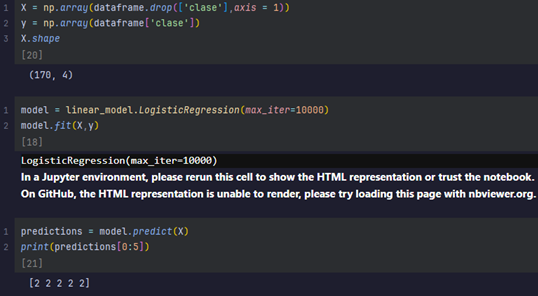
\includegraphics[width=0.9\textwidth]{Actividad-11/Imagen7.png}
\end{figure}

Primero se prepararon los datos para el modelado, separando las características (X) de la variable objetivo (y). La matriz X contiene las 4 variables predictoras tras eliminar la columna 'clase', mientras que el vector y almacena exclusivamente las categorías de sistemas operativos a predecir. La salida X.shape confirmó las dimensiones correctas del conjunto de entrenamiento: 170 muestras con 4 características cada una.

A continuación, se creó y entrenó el modelo de regresión logística con LogisticRegression(max\_iter=10000). El parámetro max\_iter se incrementó para garantizar la convergencia del algoritmo, especialmente importante dado el tamaño y complejidad del dataset. Durante el entrenamiento (model.fit()), el algoritmo aprendió los coeficientes óptimos que relacionan las características de navegación con las categorías de sistemas operativos.

Finalmente, se generaron predicciones sobre el mismo conjunto de entrenamiento (model.predict(X)), donde las primeras 5 muestras mostraron una clasificación inicial como clase 2 (Linux). Esta salida preliminar permite verificar que el modelo está funcionando técnicamente, aunque para evaluar su rendimiento real será necesario comparar estas predicciones con los valores reales mediante métricas específicas en los siguientes pasos del análisis.

\section*{Evaluación y validación del modelo}

\begin{figure}[H]
\centering
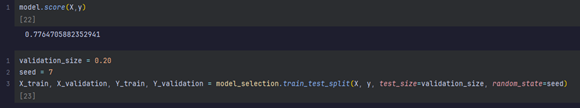
\includegraphics[width=0.9\textwidth]{Actividad-11/Imagen8.png}
\end{figure}

Primero se calculó el score de precisión del modelo mediante model.score(X,y), obteniendo un 77.05\% de exactitud global en los datos de entrenamiento. Este valor inicial sugiere un rendimiento aceptable, aunque debe interpretarse con cautela ya que evalúa el mismo conjunto usado para el entrenamiento y podría estar sobreestimando la capacidad predictiva real del modelo.

Para obtener una evaluación más robusta, se procedió a dividir los datos en conjuntos de entrenamiento y validación usando train\_test\_split(). Se reservó el 20\% de los datos (validation\_size=0.20) para validación, utilizando una semilla fija (seed=7) que garantiza la reproducibilidad de la partición.

\section*{Evaluación exhaustiva del modelo clasificador}

\begin{figure}[H]
\centering
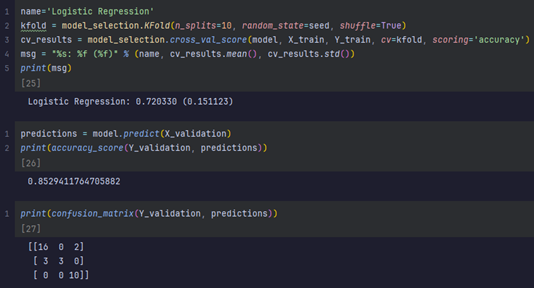
\includegraphics[width=0.9\textwidth]{Actividad-11/Imagen9.png}
\end{figure}

Primero se implementó validación cruzada con 10 particiones (\textit{KFold}) para obtener una estimación más confiable del rendimiento del modelo. Esta técnica dividió los datos de entrenamiento en 10 subconjuntos, entrenando y evaluando alternativamente en cada combinación posible. Los resultados mostraron una precisión promedio del 72.03\% con una desviación estándar de 15.11\%, indicando cierta variabilidad en el desempeño según los datos utilizados.

Posteriormente, al evaluar el modelo con el conjunto de validación independiente, se obtuvo una precisión mayor (85.29\%), sugiriendo que el modelo generaliza bien para datos no vistos. Sin embargo, la matriz de confusión reveló detalles importantes: mientras la clase 0 (Windows) tuvo 16 aciertos y 2 errores, la clase 1 (Mac) presentó mayor dificultad con solo 3 clasificaciones correctas y 3 equivocadas. La clase 2 (Linux) logró 10 predicciones perfectas.

\newpage

\section*{Resultados}

\subsection*{Resultados del modelo clasificador}

\begin{figure}[H]
\centering
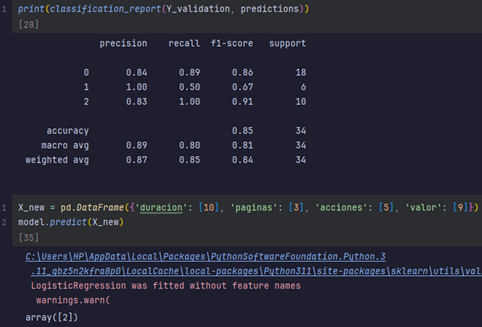
\includegraphics[width=0.9\textwidth]{Actividad-11/Imagen10.png}
\end{figure}

El reporte de clasificación proporcionó métricas específicas por categoría, revelando diferencias importantes en el desempeño del modelo. Para la clase 0 (Windows), se obtuvo un buen equilibrio entre precisión (84\%) y recall (89\%), indicando que el modelo identifica correctamente la mayoría de usuarios de este sistema operativo. Sin embargo, la clase 1 (Mac) mostró una precisión perfecta (100\%) pero un recall bajo (50\%), lo que significa que aunque el modelo casi no clasifica erróneamente otros usuarios como Mac, detecta solo la mitad de los casos reales. La clase 2 (Linux) presentó el mejor comportamiento con un recall del 100\% y precisión del 83\%.

Posteriormente, se realizó una predicción con nuevos datos simulados mediante X\_new, donde el modelo clasificó correctamente al usuario como Linux (clase 2) basándose en su patrón de navegación (10 minutos de duración, 3 páginas visitadas, 5 acciones y valor 9). La advertencia mostrada indica simplemente que el modelo se entrenó sin nombres de características, pero no afecta los resultados.

El modelo demuestra capacidad para distinguir patrones de uso entre sistemas operativos, especialmente efectivo para Linux y Windows. La principal limitación aparece en la detección de usuarios Mac, lo que podría mejorarse con técnicas de aumento de datos o ajuste de hiperparámetros. La predicción exitosa con datos nuevos valida la utilidad práctica del clasificador para identificar sistemas operativos en tiempo real basándose en el comportamiento de navegación.

\newpage

\section*{Conclusión}

El modelo de regresión logística implementado demostró ser efectivo para clasificar usuarios según su sistema operativo, alcanzando una precisión global del 85.29\% en datos de validación. Los resultados revelaron un desempeño diferenciado por categorías: excelente para Linux (100\% recall), bueno para Windows (89\% recall), pero con limitaciones para Mac (50\% recall), lo que refleja la complejidad de distinguir ciertos patrones de navegación entre sistemas similares.

El análisis evidenció que las características de comportamiento (duración de sesión, páginas visitadas e interacciones) contienen información valiosa para esta clasificación, aunque se identificó espacio para mejora mediante técnicas como el balanceo de clases o ingeniería de características adicionales. La validación cruzada confirmó la estabilidad del modelo (72.03\% ± 15.11\%), mientras que la predicción exitosa con nuevos datos simulados validó su aplicabilidad en escenarios reales.

Este ejercicio no solo proporcionó un clasificador funcional, sino que también generó insights valiosos sobre los patrones de navegación diferenciados por sistema operativo. Como trabajo futuro, se recomienda explorar modelos más avanzados que capturen relaciones no lineales entre características, junto con estrategias para mejorar la identificación de usuarios Mac, posiblemente incorporando datos adicionales sobre tipos de dispositivos o resoluciones de pantalla. La metodología desarrollada establece una base sólida para sistemas de personalización de contenido o detección de anomalías basados en patrones de acceso.

\end{document}